\documentclass[a4paper]{IEEEtran}

\usepackage[backend=bibtex]{biblatex}
\addbibresource{paper}
\usepackage{hyperref}
\usepackage{graphicx}
\usepackage{amsmath,amsfonts}
\usepackage{algorithm,algorithmicx,algpseudocode}
\renewcommand{\algorithmicrequire}{\textbf{Input:}}
\renewcommand{\algorithmicensure}{\textbf{Output:}}
\usepackage{color}
\title{Dynamic Anomaly Detection for Collective Data Via Statistical Distance}
%
\author{%
	% author names are typeset in 11pt, which is the default size in the author block
	{Ruoyu Wang{\small $~^{\#1}$}, Daniel Sun{\small $~^{*2}$}, Guoqiang Li{\small $~^{\#3}$} }%
	% add some space between author names and affils
	\vspace{1.6mm}\\
	\fontsize{10}{10}\selectfont\itshape
	% 20080211 CAUSAL PRODUCTIONS
	% separate superscript on following line from affiliation using narrow space
	$^{\#}$\,School of Software Engineering, Shanghai Jiao Tong University\\
	No.800 Dongchuan Rd. Shanghai, 200240, China\\
	\fontsize{9}{9}\selectfont\ttfamily\upshape
	%
	% 20080211 CAUSAL PRODUCTIONS
	% in the following email addresses, separate the superscript from the email address 
	% using a narrow space \,
	% the reason is that Acrobat Reader has an option to auto-detect urls and email
	% addresses, and make them 'hot'.  Without a narrow space, the superscript is included
	% in the email address and corrupts it.
	% Also, removed ~ from pre-superscript since it does not seem to serve any purpose
	$^{1}$\,solftwarewry@sjtu.edu.cn\\
	$^{3}$\,li.g@sjtu.edu.cn%
	% add some space between email and affil
	\vspace{1.2mm}\\
	\fontsize{10}{10}\selectfont\rmfamily\itshape
	% 20080211 CAUSAL PRODUCTIONS
	% separated superscript on following line from affiliation using narrow space \,
	$^{*}$\,Data61, Commonwealth Scientific and Industrial Research Organization, Australia\\
	\fontsize{9}{9}\selectfont\ttfamily\upshape
	% 20080211 CAUSAL PRODUCTIONS
	% removed ~ from pre-superscript since it does not seem to serve any purpose
	$^{2}$\,daniel.sun@data61.csiro.au
}

\begin{document}
	\maketitle
	
	\begin{abstract}
		Hackers can infiltrate networks and find their way into databases and software systems. Not only
		can they steal chunks of data and hold them for ransom, but
		also alter key information contained in those systems, setting up
		traps hard to discover and causing damages unlikely to recover.
		Although altering single record may not oblige correct value scope such that it is hard to detect, the change, especially to a subset of data, can be observed and detected in a collective
		scale. In this paper, we present a collective anomaly
		detection technique based on statistical distance. The technique
		extracts distribution similarities among data collections, and then uses the statistical distance to detect
		collective anomalies. In order to adapt to data dynamics, our technique continuously evaluates 
		metrics as evolving features. Aiming at broad generalisation, this
		technique can replace several components of our solution to further improve the
		performance of detection for various scenarios. To illustrate details of the technique
		and explore its efficiency, we case-studied a real
		world problem of click farming detection against malicious online
		sellers. The evaluation shows that the technique maps normal
		and anomalous data collections into two distinct clusters by yielding
		efficient classifiers. Those classifiers are sensitive sufficiently to
		a much smaller magnitude of data alerting, compared with real
		world malicious behaviours--that is--it is applicable in the real world. 
		
		%Hackers can infiltrate networks via any attack vector, find their way into databases and applications. Not only can they steal chunks of data and hold them for ransom, but also alter key information contained in those systems, setting up traps hard to discover and causing damages unlikely to recover. Although the influence of data altering is not significant in single data record, the change can be observed and detect in a collective scale.
		%In this paper, we present a dynamic collective anomaly detection technique based on statistical distance. The technique extracts distribution similarities among data collections, reducing collective anomalies into point anomalies. It dynamically calculate metrics which is adaptive to the slightly evolving features. This technique provides a basic solution where several components can be replaced by other scenario specific ones, further improving the performance of detection.
		%To illustrate details of the technique and explore its efficiency, we applied the algorithm into a real world problem of click farming detection against malicious online sellers. The evaluation shows that the technique maps normal and anomalous data collections into two distinct clusters, yielding efficient classifiers. And those classifiers are sensitive enough to a much smaller magnitude of manipulation compared with real world malicious behaviours.
	\end{abstract}
	
	\section{Introduction}
		Major improvements in data acquisition, transmission and storage are driving increased data availability and affordability. Currently, there are totally 2.7ZB data in the digital universe~\autocite{bigDataStatistics} and the growing speed is doubling every two years.
		%In Facebook, there is about 100 terabytes of data uploaded every day~\cite{bigDataFacebook}.
		%Big data analysis has been widely adopted in scientific experiments~\autocite{nothaft2015rethinking}, electric business~\autocite{bronson2015open,sumbaly2013big,chen2016realtime}, healthcare~\autocite{groves2016big}, governments~\autocite{kim2014big} and many other fields.
		%
		It has already been and will be much harder in the future to harness the exploding volumes of data which is now pervasive leading to many problems in data management and engineering, threatening trustworthiness and reliability of data flows inside working systems.
		
		Data error rate in enterprises is approximately 1\% to 5\%, and for some, even above 30\%~\autocite{saha2014data}.
		In 2016, according to the research by Tricentis~\cite{softwareFailure}, software failures cost \$1.1 trillion US dollars in total and those at 363 investigated companies affected 4.4 billion customers, causing the total lost time of more than 315.5 years. And it takes more than 45\% of total expense to eliminate those errors~\cite{pawar2016software}. System configuration problems, as a matter of fact, also draw scratches to the messy picture. They take even dominant places in failures in large distributed clusters~\cite{xu2015systems}.
		
		Those data anomalies may arise due to both internal and external reasons with respect to a certain system. On one hand, components inside the system may generate problematic source data. For example, in a sensor network, some sensors may generate erroneous data when it experiences power failure or other extreme conditions~\autocite{rassam2014adaptive}. Data packages will be lost if sensor nodes fail to connect to network or some sensor hub goes down~\autocite{herodotou2014scalable}. Also, human operators act as a heavily vulnerable part to bugs and mistakes. Some insiders even deliberately modify system configurations for malicious compromises~\autocite{schuster2015vc3}. A study~\autocite{humanError} found that 65\% of organizations state that human errors are the main  cause of data problems.
		
		On the other hand, data manipulation~\autocite{dataManipulation} from outside hackers composes another potential threat of data quality and reliability. \textit{Data Manipulation} here, according to a NSA definition, refers to that ``hackers can infiltrate networks via any attack vector, find their way into databases and applications and change information contained in those systems, rather than stealing data and holding it for ransom''.
		% Take an example of Apache Hadoop, Hadoop's security issues has long been discussed within communities and industry~\autocite{sharif2015current,terzi2015survey,jam2014survey,sharma2014securing}. As is shown in Figure~\ref{fig:hadoop-security}, the two basic vulnerabilities: \textit{lack of access control} and the \textit{absence of encryption} expose the entire cluster to dangerous threats. Data flows can be intercepted and modified; services can also be altered and blocked~\autocite{huang2014denial}. Although there are several frameworks(e.g. Kerberos, Sentry, Knox etc.) and algorithms providing basic protection~\autocite{zheng2017towards,sikdar2017spatio,xu2016high,yu2015enhancing,cohen2014towards}, clever attackers can always bypass the barriers and sneak into the core of data pipelines. Several approaches are developed as sentinels to detect probable infiltrations. However, these approaches are not able to detect corrupted data under carefully planned manipulations. Nor can they figure out the exact reasons and recover the original records. 
		If data inside the system is compromised, they will severely affect mining and learning algorithms and further change the final decision given by the entire system. In 2013, hackers from Syria put up fake reports via Associated Press' Twitter account and caused a 150-point drop in the Dow~\cite{SyriaHacker}.
		% To locate and diagnose anomalies in data pipelines under carefully planned and disguised data manipulations are still in demand by industry and academia.
		
		%\begin{figure}[!t]
		%	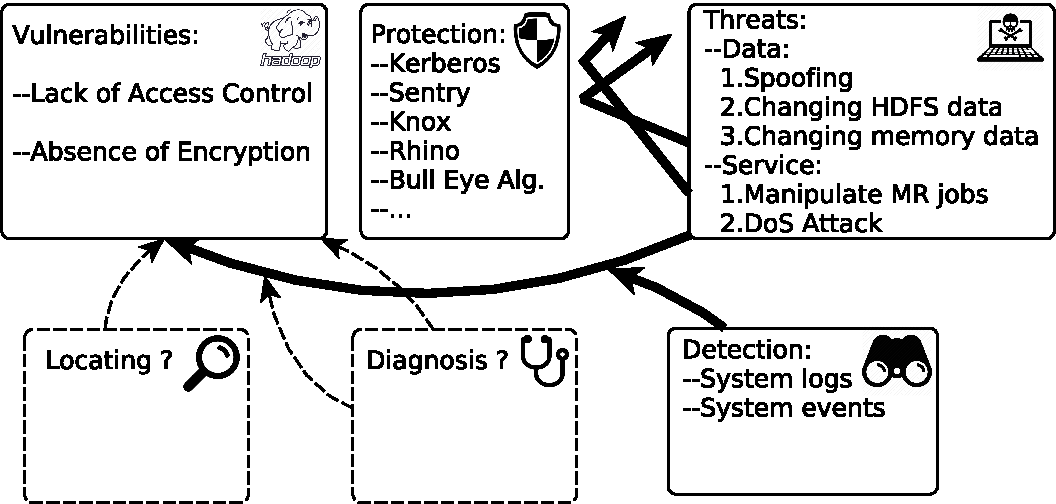
\includegraphics[width=\linewidth]{fig/HadoopSecurity}
		%	\caption{Security Issues of Hadoop Clusters}
		%	\label{fig:hadoop-security}
		%\end{figure}
		
		However, from the aspect of data itself, we can still detect malicious data manipulation behaviours.
		According to our observation, typical data manipulations on numerical data will lead to a drift or distortion of its original distribution. With the reshaping measurable, we can enclose data collections with similar distribution forms inside the same cluster and filter out those strange shaped ones. In this paper, we adopt Jensen-Shannon divergence as the similarity measurement among different distributions. Comparing with a estimated ground truth, each data collection can be mapped to a single real number within a definite interval. Then a gaussian classifier can be applied to detect outliers derived from manipulated data. To automatically calculate adaptive threshold for the classifier, we keep two evidence sets for both normal points and anomalies, taking advantage of the property provided by Jensen-Shannon divergence. And those evidence sets are set to be slide windows to keep up to the evolving features in dynamic scenarios.
		%For example, a Taobao online seller's transaction records(see section~\ref{sec:exp-methodology}) can be ``click farmed'' to increase the volume of sales. Fig.~\ref{fig:example-ecdf} shows the sales distribution within one day. The curve for cheated data is emulated according to a popular method for click farming. It can be observed that there exists clearly a gap between these two distributions. 		
		%For example, in a sampled data set from Melbourne city pedestrian volume along main streets\footnote{https://data.melbourne.vic.gov.au/Transport-Movement/Pedestrian-volume-updated-monthly-/b2ak-trbp}, 20\% records were randomly selected and modified, the value set as a tenth of the original. The empirical cumulative distribution function of the two data sets are shown in Fig.~\ref{fig:example}, where there is clearly a gap between these distributions.
		Details of the technique are put together with a real world problem of ``Click Farming'' and had been evaluated on both raw and synthetic data sets corresponding to the problem, demonstrating the correctness and effectiveness of the technique.
		
		The rest of the paper is organised as follow: Section~\ref{sec:related-work} states related works on data anomaly detection and describes a real world problem. Section~\ref{sec:preliminaries} introduces statistical distance. Details of the technique are proposed in section~\ref{sec:algorithm-details}. Section~\ref{sec:evaluation} presents evaluation results and further findings of the algorithm. And all contents are concluded in section~\ref{sec:conclusion}.
	
	\section{Related Work}\label{sec:related-work}
		\subsection{Data Anomaly Detection}
			Anomaly detection, also known as outlier detection, has been studied for a long time and discussed in diverse research domains, such as fraud detection, intrusion detection, system monitoring, fault detection and event detection in sensor networks. According to a comprehensive study in~\cite{chandola2009anomaly}, anomaly detection algorithms deal with input data in the form of points(or records), sequences, graphs and spatial relationships, where point data is the simplest and well studied, others are attracting more attention in new studies.
			
			Prevalent anomalies can be classified into \textit{Point Anomalies}, \textit{Contextual(or Conditional) Anomalies} and \textit{Collective Anomalies}. Point anomalies refers to an individual data instance that is considered anomalous with respect to others. But if it is anomalous only in certain circumstances or a specific context, the instance is regarded as contextual anomaly. If a group of related data(e.g. a segment of sequence) instances is anomalous with respect to other groups in the data set(e.g. the entire sequence), it is called a collective anomaly~\cite{goldberger2000components}.
			
			Detection approaches can be categorized into three types according to whether data is labeled: \textit{Supervised}, \textit{Semi-Supervised} and \textit{Unsupervised} anomaly detection. As the name suggests, supervised detection methods train models on completely labeled data while unsupervised detection leverages data without any labeling. Semi-supervised detection approaches train model on data that has labeled instances for only the normal class. Supervised detection is commonly applied when both normal and anomalous data can be obtained.~\cite{fujimaki2005approach} When it comes to the circumstances that anomalous data is hard to obtain or there exist too many diverse types of anomalies to enumerate, semi-supervised or unsupervised approaches are usually taken into consideration.
			
			To make the final decision, detection algorithms mostly yield a score from each input instance, denoting how likely it is anomalous. The algorithm then selects top few as anomalies or compare the score with a threshold. Or, detection algorithms output a label on each instance, then decide whether each label belongs to the normal class.
			
			Currently, distance based~\cite{cao2014scalable,cao2017multi} and feature evolving algorithms~\cite{masud2013classification,li2015discovery,shao2014prototype} algorithms seize most attention. Others adopted tree isolation~\cite{zhang2017lshiforest}, model based~\cite{yin2016model} and statistical methods~\cite{zhu2002statstream} in certain applications.
			
			To detect collective anomalies,~\cite{caudell1993adaptive} adopted the \textit{ART(Adoptive Resonance Theory)} neural networks to detect time-series anomalies. \textit{Box Modeling} is proposed in ~\cite{chan2005modeling}. And \textit{Longest Common Subsequence} was leveraged in ~\cite{budalakoti2006anomaly} as similarity metric for symbolic sequence. Markovian modeling techniques are also popular in this domain\cite{ye2000markov,warrender1999detecting,pavlov2003sequence}. \cite{yu2015glad} depicted groups in social media as combinations of different ``roles'' and compare groups according to the proportion of each role within each group.
			
		\subsection{Real World Problem: Click Farming Detection}\label{sec:related-realworld}
			Since the establishment of Taobao in 2003, the online business platform has been growing from the rookies in the market to the No.1 service provider in B2B and B2C markets, possessing a market share of 50.6\% to 56.2\% in China by 2016~\cite{iresearch2016b2c}. Currently, there are more than 9.4 million sellers in Taobao, providing more than 1 billion different products. Under the super-pressure from massive competition, most of the sellers choose to use some cheating techniques to raise reputation and product sale volumes, then improve rankings in search lists.
			
			The most popular approach to manipulate transaction and reputation data is \textit{Click Farming}, where sellers use a large number of buyer accounts to create fake transaction records and give high remarks on products. Professional click farmers are usually well organized groups or companies containing thousands of people. Leaders of such groups receive orders from sellers and assign tasks to other members to create fake transactions. Some companies even develop professional applications that can be deployed on common PCs to improve productivity~\cite{zhao2016on}.
			
			A research performed in China showed that 81.9\% of the people investigated had heard of the behaviour of click farming, 51.2\% of them had seen people around them click farmed and 18.9\% of them had experience of click farming themselves~\cite{yan2015report}. American researchers reported in 2015 that over 11000 sellers were detected to have click farmed records and only 2.2\% of 4000 investigaed sellers had been penalized because of the cheating attempts~\cite{netease2015research}.
			
			Current detection techniques for click farming mainly focus on user behaviours, such as browsing frequencies and periods, most common purchasing time, favourite products, remarks and whether they communicate with sellers~\cite{simpleDetection}. Those techniques require the platform to keep lots of records and user features. However, the detection can be easily bypassed by trained workers and some well programmed applications.
			
			Although it is hard to classify users as honest and malicious, we can still find clues from the sellers' aspect. For normal sellers, their customers are usually similar since choices of products are seldom changed. Therefore, the distribution of transactions in a fixed period of time, say one day, is relatively stable. No matter how much alike between the employed users or robots with honest users, the fake transaction records will always cause a bias or distortion of the original transaction distribution. To better observe the problem, we downloaded a real world data set containing Taobao online sellers' transaction records(see section~\ref{sec:exp-methodology}) and emulated the circumstances if it had been click farmed. Figure~\ref{fig:example-ecdf} shows the difference between one daily distribution with and without click farming.
			
			\begin{figure}[!t]
				\centering
				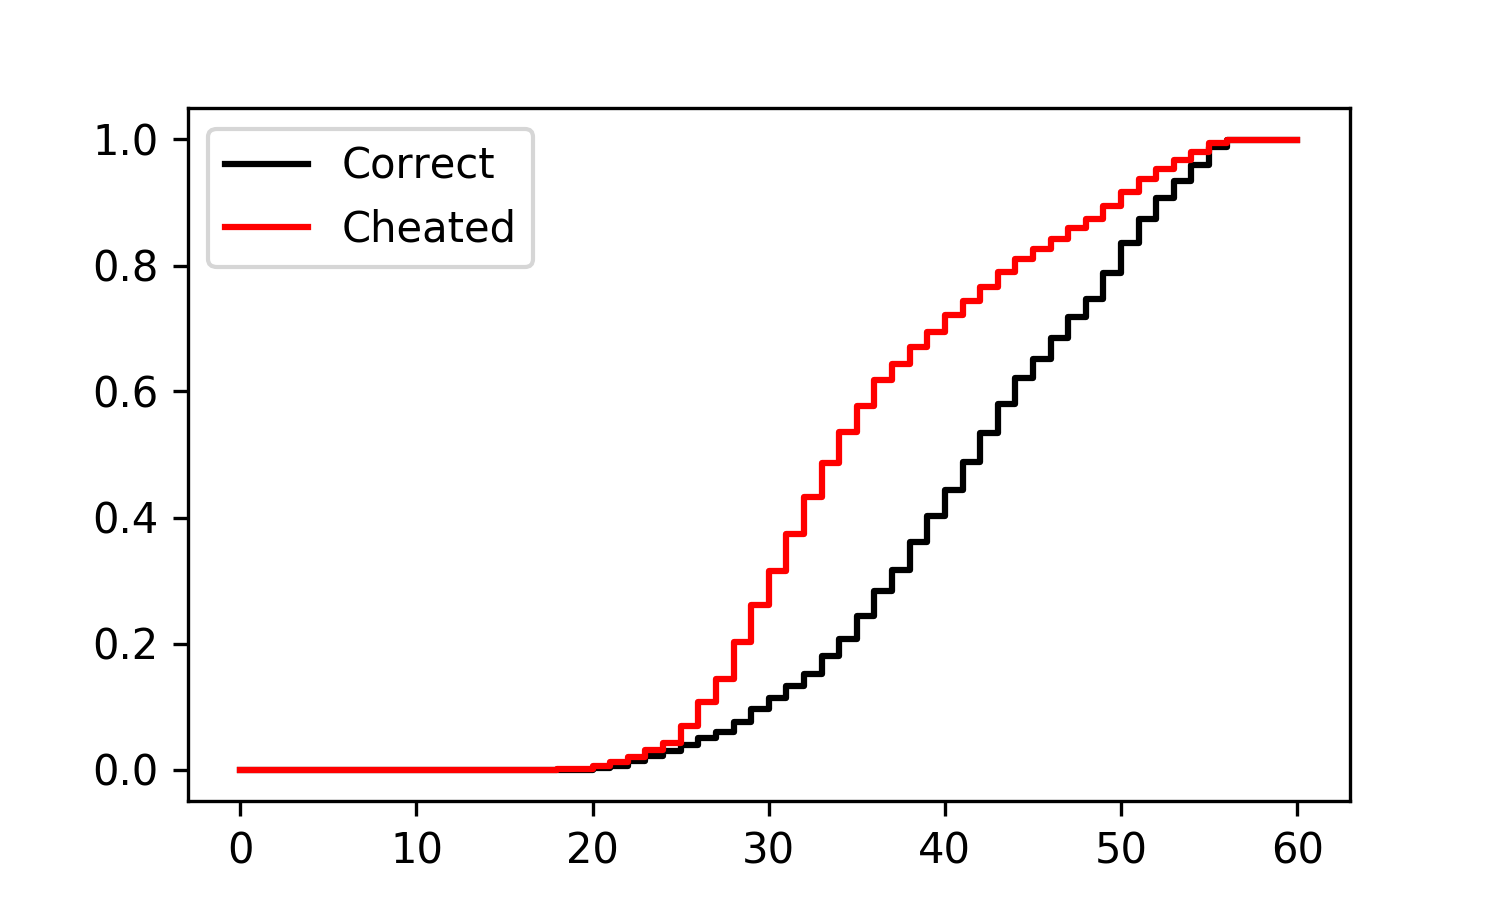
\includegraphics[width=\linewidth]{fig/ExampleEcdf.png}
				\caption{Example Cumulative Distribution Function of Original And Click Farmed Daily Transaction Data}
				\label{fig:example-ecdf}
			\end{figure}
			
			Thus, if we can measure the similarity between different transaction distributions, there is still a chance for us to detect dishonest sellers.
			
	\section{Preliminaries}\label{sec:preliminaries}
		Statistical divergence, also called statistical distance, measures the similarity between two or more distributions.
		% This mathematical tool can be adopted in our solution to map distributions into one dimensional points, turning collective anomaly detection problem into point anomaly detection problem. Then a concrete point anomaly detection classifier can be used to find out the cheaters.
		Mathematically, statistical divergence is a function which describes the ``distance'' of one probability distribution to the other on a statistical manifold. Let $S$ be a space of probability distributions, then a divergence is a function from $S$ to non-negative real numbers: 
		\begin{equation}
			D(\cdot || \cdot): \mathbb{S} \times \mathbb{S} \rightarrow \mathbb{R^+}
		\end{equation}
		
		Divergence between two distributions $P$ and $Q$, written as $D(P||Q)$, satisfies:
		
		\begin{enumerate}
			\item $D(P||Q) \ge 0, \forall P, Q \in S$
			\item $D(P||Q) = 0$, if and only if $P=Q$
		\end{enumerate}
		
		For our purposes, we do not require the function $D$ to have the property: $D(P||Q) = D(Q||P)$. But we do need it to be true that if $Q$ is more similar with $P$ than $U$, then $D(Q||P) < D(U||P)$. There are many ways to calculate divergence, such as f-divergences, M-divergences and S-divergences.
		%Some of them provides better properties which brings conveniences to the design and implementation of our approach. 
		Considering that the sensitivity and computational cost of the function are directly related to the performance of our technique, we chose Jensen-Shannon divergence which is derived from Kullback-Leibler as the measurement.
		
		\subsubsection{Kullback-Leibler Divergence}
		Let $P,Q$ be discrete probability distributions, $Q(i)=0$ implies $P(i)=0$ for $\forall i$, the \textit{Kullback-Leibler Divergence} from $Q$ to $P$ is defined to be:
		
		\begin{equation}
		KLD(P||Q) = \sum_{Q(i)\ne 0} P(i)log\Big(\frac{P(i)}{Q(i)}\Big)
		\end{equation}
		
		For $P,Q$ being continuous distributions:
		
		\begin{equation}
			KLD(P||Q) = \int_{-\infty}^{+\infty} P(x)log\frac{P(x)}{Q(x)}dx
		\end{equation}
		
		\subsubsection{Jensen-Shannon Divergence}
		Let $P,Q$ be discrete probability distributions, \textit{Jensen-Shannon Divergence} between $P$ and $Q$ is defined to be:
		
		\begin{equation}
		JSD(P||Q) = \frac{1}{2}KLD(P||M) + \frac{1}{2}KLD(Q||M)
		\end{equation}
		where $\displaystyle M = \frac{1}{2}(P+Q)$.
		
		A more generalized form is defined to be:
		
		\begin{equation}
		JSD_{\pi_1, \dots, \pi_n}(P_1, \dots, P_n) = \sum_{i=1}^{n}\frac{1}{\pi_i}KLD(P_i||M)
		\end{equation}
		where $\displaystyle M = \sum_{i=1}^{n}\frac{1}{\pi_i}P_i$ and $\displaystyle \sum_{i=1}^{n}\frac{1}{\pi_i} = 1$.
		
		Jensen-Shannon divergence has some fine properties:
		\begin{enumerate}
			\item $JSD(P||Q) = JSD(Q||P), \forall P, Q\in \mathbb{S}$.
			\item $0 \le JSD_{\pi_1, \dots, \pi_n}(P_1, \dots, P_n) \le log_k(n)$. If a $k$ based algorithm is adopted.
			\item To calculate $JSD(P||Q)$, it need not necessarily to be true that $Q(i)=0$ implies $P(i)=0$.
		\end{enumerate}
	
	\section{Statistical Detection}\label{sec:algorithm-details}
		Diverse data sets in the real world show certain structures caused by hidden patterns or relationships among records in a collection of data. For example, the traffic volume in the highway and the business transaction records, they may show a relatively stable distribution in the daily scale. Manipulation on those data(e.g. Fig~\ref{fig:example-ecdf}) results in a drift or distortion of the distribution, which can be captured to trigger the alarm. Main idea of the solution is simple. But there are several difficulties to be solved in the design and implementation of the technique:
		
		\begin{enumerate}
			\item Are the corresponding one-dimensional points distinguishable after mapping form normal and anomalous distributions? And which classifier is efficient towards those points?
			\item Is there a general approach that can effectively depict different distributions in various circumstances?
			\item What classifier specific metric should be adopted to filter out anomalies? Can it be further optimized?
			\item Online shops are often in the process of expanding or dwindling. Thus the sales distribution will slightly change as time goes on. How to make the technique adapt to these drifting distributions?
		\end{enumerate}
		
		\ref{sec:alg-basic} answers the first question and introduces a basic framework of our technique. The second question is studied in~\ref{sec:alg-histogram}. \ref{sec:alg-threshold} gives an analysis about adaptive metric that minimizes total error. And a dynamic framework is proposed in~\ref{sec:alg-dynamic}.
			
		\subsection{Divergence-Based Collective Anomaly Detection}\label{sec:alg-basic}
			From section~\ref{sec:preliminaries} we know that statistical divergence only provides a distance between two or more distributions. In a set of data collections, we can only draw a complete graph that each node denotes one certain collection and each edge refers to the divergence of two data collections. From the graph we can find some points that have apparently larger distances with most of other points and return them as anomalies. This may work if anomalous ones do not compose a large proportion of all points. However the procedure will be too complicated to work out with large amounts of instances. 
			
			Otherwise we need a frame of reference and yielding absolute distances rather than the relative ones. Therefore, we should keep an evidence set $\mathbb{E}$ which consists of several already known correct distributions. Then the real distribution can be estimated by averaging all distributions in $\mathbb{E}$. This process is similar to the parameter estimation within a certain sample set. Let $M$ denote the estimated population distribution, then we can measure the statistical distance with respect to $M$ for every distribution $D$ inside or outside $\mathbb{E}$, yielding absolute distances. 
			
			Fig.~\ref{fig:raw-hist-1st} and~\ref{fig:raw-hist-2nd} in section~\ref{sec:exp-raw} show the result of the above process. Red dots refer to the distances calculated from normal transaction data collections, blue and green ones are from click farmed collections. Clearly, distances of normal data collections assembles together around a small value while anomalous ones are distributed around a larger distance value. Intuitively, a simple gaussian classifier can be suitable here to discover anomalous data points. The basic framework of the algorithm is shown in Algorithm~\ref{alg:static}:
			
			\begin{algorithm}[!t]
				\caption{Basic Classification}
				\label{alg:static}
				\begin{algorithmic}[1]
					\Require Evidence set $\mathbb{E} = \{D_1, \dots, D_n\}(n\ge2)$; New data collection $D'$
					\Ensure Whether $D'$ is anomalous
					\For{$i \gets 1$ to $n$ do}
					\State $P_i \gets$ the distribution of $D_i$
					\EndFor
					\State $M \gets \frac{1}{n}\sum_{i=1}^{n}P_i$\label{line:population-estimation}
					\For{$i \gets 1$ to $n$ do}
					\State $J_i \gets JSD(P_i||M)$
					\EndFor
					\State $N \gets$ normal distribution estimated from $J_1, \dots, J_n$
					\State $P' \gets$ distribution of $D'$
					\State $J' \gets JSD(P'||M)$
					\State $p \gets$ probability density of $J'$ in $N$
					\If{$p <$ Threshold}
					\State \textbf{Return} True
					\Else
					\State \textbf{Return} False
					\EndIf
				\end{algorithmic}
			\end{algorithm}
			
			Let $\mathbb{S}$ be set of the daily transaction collections, if $\mathbb{E}$ is already given, we can run the algorithm with $\mathbb{E}$ and $\forall D \in \mathbb{S}$ and discover the anomalies. Although it is convenient to compute $JSD(P_1, \dots, P_n, P')$ instead of $JSD(P_1||M), \dots, JSD(P_n||M), JSD(P'||M)$, it is not viable for classification. Jensen-Shannon divergence of $n+1$ distributions will dilute the affection of the abnormal one, in which case the difference between $P'$ being normal and anomalous will become subtle when $n$ goes very large. For example, suppose $P(1) = P(2) = P(3) = \frac{1}{3}$ and $P'(1) = \frac{1}{6}, P'(2) = \frac{1}{3}, P'(3) = \frac{1}{2}$, then $JSD(P||P') \approx 0.023$ and $JSD(P, P, P, P') \approx 0.017$.
			
			According to the property of statistical divergence, we can infer that the true distribution of JSDs calculated form normal data collections are close to but not exactly a gaussian distribution $N(\mu, \sigma)$ since for each point, there are both definite upper and lower bounds instead of infinities. Therefore, $\mu$ should be slightly larger than zero. The reason why $\mu$ cannot be exactly zero is hidden in line~\ref{line:population-estimation}.
			For $\mu = 0$ if and only if $J_i = 0$ for $\forall i = 1, \dots, n$, which is equivalent to $P_i = P_j$ for $\forall i, j = 1, \dots, n$. And, $\lim_{n\rightarrow+\infty}P(P_i = P_j,\forall i, j = 1, \dots, n)=0$. Thus it is highly unlikely for real world data sets to have $u=0$.
			%$M$ takes into consideration all existing values in every distribution sample and averages corresponding probabilities. Thus for a large $|S|$, $M$ may highly probably contains entries that does not exist in $P_i$ and certain probability entries in $M$ may vary from that in $P_i$. For a concrete example, suppose $P_1(1)=0.5, P_1(2)=0.3, P_1(3)=0.2$; $P_2(1) = 0.3, P_2(2) = 0.4, P_2(3) = 0.3$; $P_3(1)=0.3, P_3(3)=0.5, P_3(4)=0.2$, then $M(1) = \frac{11}{3}, M(2)=\frac{7}{3}, M(3)=\frac{10}{3}, M(4)=\frac{2}{3}$. None of $P_1, P_2, P_3$ is the same with $M$.
		
		\subsection{Distribution Histogram}\label{sec:alg-histogram}
			Not all data collections can be assumed subject to known distributions. Parameter approximation will probably lead to errors far beyond our expectation. For example, the distribution of vehicle volume in the highway may not correspond to any of the prevalent distribution model. Few assumption of parameters can be made in advance on such data. For the sake of generality, non-parametric estimation should be applied.
			
			Surely, the kernel density estimation approaches will give a smooth, continuous distribution curve under on any sampled data. The computational cost will be much higher than applying a coarse histogram approximation.
			Moreover, even if we applied a distribution model upon a collection of sampled data, yielding more accurate results, the computation of divergence will be much more complex on continuous functions than discrete distributions.
			
			Histogram methods can not only be applied to non-parametric distributions, but also to miscellaneous data types. From a general point of view, as long as there exits a function mapping the input data instance into a subset of real numbers, this data collection can be counted into a histogram. For example, date, time and single characters.
			
			In order to generate a accurate approximation, step size is the most important parameter the algorithm should determine. If the size is too small then the resulting histogram will be over fitting; but if the size is too large then the estimation will be too coarse to depict the original shape. According to statistics theory, when dealing with a sample size of $k$, a step size of 
			
			\begin{equation}\label{equ:step-size}
				l = c \sigma k^{-0.2}
			\end{equation}
			
			will give a best partition, where $c$ is a constant relative to the shape of distribution(e.g. for normal distribution, $c=1.05$). For data sets with a large number of elements, a random sampling method, such as Monte-Carlo method, can be applied to speed up the estimation procedure.
			
		\subsection{Threshold}\label{sec:alg-threshold}
			One important factor in the algorithm is the value of threshold. A higher threshold rejects more instances, improving the sensitivity of anomalous data while increasing the number of false alarms. A lower threshold provide higher true negative rates yet neglecting more possible threats.
			
			A naive but prevalent approach is to set a fixed value as threshold. This approach is easy to implement and may give satisfying results in specific cases. However, a fixed threshold requires specific analysis in the certain scenario, manual observation and tuning of parameters, which involves lots of human labour. The rule of ``$3 \sigma$'' can be used to automatically determine a threshold. But as a rigid metric, it is merely an estimation of a suitable boundary considering average situations, which is far from optimal when concrete data is provided. It would be either higher than the optimum if anomalous data lies far away from the cluster consisting normal data records, or lower than the optimum if the anomalies sit more within the boundary.
			
			\begin{figure}[!t]
				\centering
				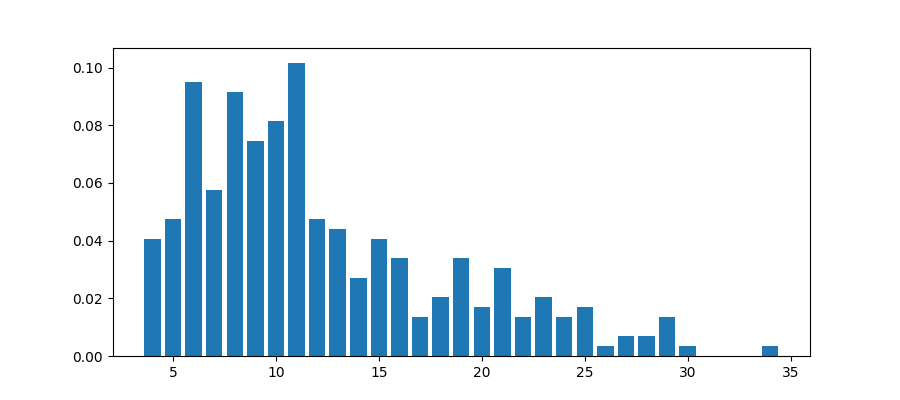
\includegraphics[width=\linewidth]{fig/JSD-Dist.png}
				\caption{Distribution of JSD values for everyday data collection. It can be approximately regarded as a gaussian distribution.}
			\end{figure}
			
			However, applying divergence as the distance measurement among data collection distributions provides a fine property. That is, divergences of normal data collections assemble together, forming a quasi-gaussian distribution. And those of anomalies also form a quasi-guassian distribution which lies in the right-hand-side interval on the real number axis. As a result of further observation, however, true distribution of both JSDs derived from normal and anomalous data collections may differ a little more from the standard gaussian than the expected estimation error. That is due to the unknown randomness within real world data. Few assumptions can be applied in real world data sets, let alone data volume is sometimes relatively low. This topic is out of the domain discussed in this paper and we here only introduce the technique instead of the specific distribution model. However, in the scenarios that better models can be calculated, distributions here can be replaced to produce better results. For the simplicity of our proposal, we assume the distributions of JSDs to be gaussian.
			%the divergence of anomalous data collections also assemble to be a quasi-normal distribution, since statistical distance has been restricted by a strict upper bound.
			
			\textbf{[Better give a Histogram drawing JSD distribution]}
			
			\begin{figure}[!t]
				\centering
				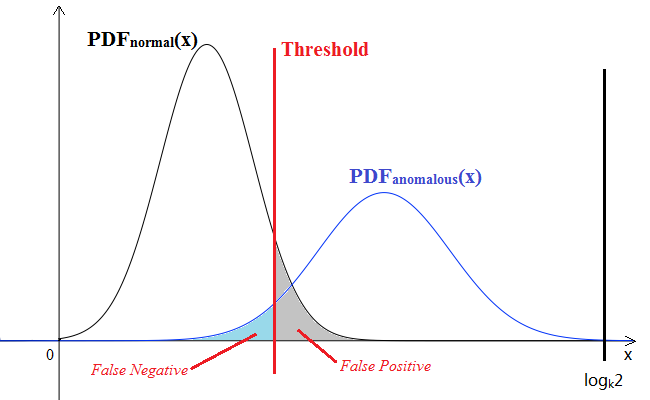
\includegraphics[width=\linewidth]{fig/ExampleThreshold.png}
				\caption{Threshold can be determined either by a probability density value, or a radius from the centre. In the scenario shown in the figure, the threshold can be determined by the position between two means of the distribution, denoted as ``T'' here. This form of threshold can also be applied to other types of distributions even there is no intersection between these two.}
				\label{fig:example-threshold}
			\end{figure}
			
			As shown in Fig~\ref{fig:example-threshold}, the black curve($PDF_{normal}(x)$) displays the probability density function(PDF) fitting those JSDs calculated from normal data collections; the blue curve($PDF_{anomalous}(x)$) displays the PDF derived from anomalous data collections. Threshold is chosen to minimize total errors(False Negative and False Positive).
			
			Suppose:
			
			\begin{align}
				PDF_{normal}(x) &\approx N(\mu_n, \sigma_n)\\
				PDF_{anomalous}(x) &\approx N(\mu_a, \sigma_a)
			\end{align}
			
			Then the optimal threshold $T$ is:
			
			\begin{equation}\label{equ:linear-weight}
				\small
				\begin{split}
					T &= \mathop{\arg\min}_{T} \int_{0}^{T}PDF_{anomalous}(x)dx +
					 \int_{T}^{log_k2}PDF_{normal}(x)dx\\
					& \approx \mathop{\arg\min}_{T}
					\int_{-\infty}^{T}
					\frac{e^{-\frac{(x - \mu_a)^2}{2\sigma_a^2}}}{\sqrt{2\pi} \sigma_a}dx
					+ \int_{T}^{+\infty}
					\frac{e^{-\frac{(x - \mu_n)^2}{2\sigma_n^2}}}{\sqrt{2\pi} \sigma_n}dx\\
					& = \frac{\mu_n\sigma_a + \mu_a\sigma_n}{\sigma_a + \sigma_n}
				\end{split}
			\end{equation}
			
			According to equation(\ref{equ:linear-weight}), threshold value can be automatically determined. The optimal threshold will minimize total errors, yielding an optimal outcome. The only requirement for this technique is another evidence set containing data point derived from anomalous data collections.
			
			However, this is not accurate enough, since equation(\ref{equ:linear-weight}) implicate an assumption that the chances are the same for a new data collection to be either anomalous or not. If we can determine the probability for a new data collection to be anomalous in any segment of data sequence, the equation should be modified as:
			
			\begin{equation}\label{equ:linear-balanced}
				\small
				\begin{split}
					T & = \mathop{\arg\min}_{T} \alpha\int_{0}^{T}PDF_{anomalous}(x)dx +
				(1-\alpha)\int_{T}^{log_k2}PDF_{normal}(x)dx\\
					& \approx \mathop{\arg\min}_{T}
					\alpha\int_{-\infty}^{T}
					\frac{e^{-\frac{(x - \mu_a)^2}{2\sigma_a^2}}}{\sqrt{2\pi} \sigma_a}dx
					+ (1-\alpha)\int_{T}^{+\infty}
					\frac{e^{-\frac{(x - \mu_n)^2}{2\sigma_n^2}}}{\sqrt{2\pi} \sigma_n}dx
				\end{split}
			\end{equation}
			
			Where $\alpha$ is the anomaly probability. Equation(\ref{equ:linear-balanced}) is much more complicated than (\ref{equ:linear-weight}). It can be reduced to a quadratic equation. But may not have real roots in some cases.
			
			Section~\ref{sec:exp-threshold} compares some estimations for optimal threshold under a real world circumstance. It shows the difference among calculators and the scenario that equation~\ref{equ:linear-balanced} outperforms others.
			
			%From another point of view, equation (\ref{equ:linear-weight}) can be regarded as a weighted averaging between two mean value: $\mu_n$ and $\mu_a$. From this aspect, we can derive some similar approximations:
			
			%\begin{align}
			%	T &= \frac{\mu_n \sqrt{\sigma_a} + \mu_a \sqrt{\sigma_n}}{\sqrt{\sigma_a} + \sqrt{\sigma_n}}
			%	\label{equ:sqrt-weight}\\
			%	T &= \frac{\mu_n \sigma_a \sqrt{-ln(1 - \alpha)}
			%		+ \mu_a \sigma_n \sqrt{-ln\alpha}}
			%	{\sigma_a \sqrt{-ln(1 - \alpha)} + \sigma_n \sqrt{-ln\alpha}}
			%	\label{equ:sqrt-log-add-weight}\\
			%	T &= \frac{\mu_n \sqrt{|ln\big[\sigma_a (1 - \alpha)\big]|}
			%		+ \mu_a \sqrt{|ln(\sigma_n \alpha)|}}
			%	{\sqrt{|ln\big[\sigma_a (1 - \alpha)\big]|} + \sqrt{|ln(\sigma_n \alpha)|}}
			%	\label{equ:sqrt-log-combined-weight}
			%\end{align}
			
			%Due to the restriction sample capacity, the replacement of JSD distributions by guassian distribution may lose too much accuracy. Compared with equation (\ref{equ:sqrt-weight}), (\ref{equ:sqrt-log-add-weight})and (\ref{equ:sqrt-log-combined-weight}), (\ref{equ:linear-balanced}) may not give a best result.
		
		\subsection{Dynamic DCAD}\label{sec:alg-dynamic}
			In Algorithm~\ref{alg:static}, there is a hidden assumption that it regards every data collection to be sampled from a static population. That is to say the seller will never change his or her products and customer volume always remain the same. In most cases, real world data is always in the process of evolution and fluctuation. Online shops are often in the process of expanding or dwindling. Thus the sales distribution will slightly change as time goes on. Therefore, the algorithms should automatically adapt to the trend at any time. To meet the need, a sliding window technique has been applied to the basic algorithm frame work. Considering discussion in section~\ref{sec:alg-histogram} and~\ref{sec:alg-threshold}, a dynamic version is proposed as follow:
			
			\begin{algorithm}[!ht]
				\caption{Dynamic DAD}
				\label{alg:dynamic}
				\begin{algorithmic}[1]
					\Require Normal evidence set $\mathbb{E}_N = \{D_{N_1}, \dots, D_{N_n}\}$ by given order; Anomalous evidence set $\mathbb{E}_A = \{D_{A_1}, \dots, D_{A_m}\}$ by given order; New data collection $D'$; Estimated anomalous probability $\alpha$
					\Ensure Whether $D'$ is anomalous
					\For{$i \gets 1$ to $n$}
						\State $P_{N_i} \gets$ histogram of $D_{N_i}$\label{line:hist-1}
					\EndFor
					\For{$i \gets 1$ to $m$}
						\State $P_{A_i} \gets$ histogram of $D_{A_i}$\label{line:hist-2}
					\EndFor
					\State $P' \gets$ histogram of $D'$
					\State $M \gets \frac{1}{n}\sum_{i=1}^{n}P_{N_i}$
					\For{$i \gets 1$ to $n$}
						\State $J_{N_i} \gets JSD(P_{N_i}||M)$
					\EndFor
					\For{$i \gets 1$ to $m$}
						\State $J_{A_i} \gets JSD(P_{A_i}||M)$
					\EndFor
					\State $J' = JSD(P'|||M)$
					\State $(\mu_N, \sigma_N) \gets$ estimated from $\{J_{N_1}, \dots, J_{N_n}\}$\label{line:gaussian-1}
					\State $(\mu_A, \sigma_A) \gets$ estimated from $\{J_{A_1}, \dots, J_{A_m}\}$\label{line:gaussian-2}
					\State $T \gets$ proper threshold derived from $(\mu_N, \sigma_N)$, $(\mu_A, \sigma_A)$ and $\alpha$
					\If{$J' < T$}
						\State $E_N \gets E_N \backslash \{D_{N_0}\} \cup \{D'\}$\label{line:update-normal-evidence}
						\State \textbf{Return} False
					\Else
						\State $E_A \gets E_A \backslash \{D_{A_0}\} \cup \{D'\}$\label{line:update-anomalous-evidence}
						\State \textbf{Return} True
					\EndIf
				\end{algorithmic}
			\end{algorithm}
			
			Algorithm~\ref{alg:dynamic} uses $\mathbb{E}_N$ and $\mathbb{E}_A$ as two sliding windows, keeping up with latest trend of both normal and anomalous features. Thus, the two window sizes $n$ and $m$ cannot be too large. Otherwise the evolving features will be flattened and aligned to the older ones. For the sake of estimation accuracy, they cannot be too small either. The size should refer to ratio of both data updates and feature evolution.
			
			Note that line~\ref{line:hist-1} and~\ref{line:hist-2} can be replaced by other estimation methods if better assumptions can be made. Line~\ref{line:gaussian-1} and~\ref{line:gaussian-2} can be replaced by other models for more accuracy. Line~\ref{line:update-normal-evidence} and~\ref{line:update-anomalous-evidence} update the evidence sets, replacing the most outdated one, moving the sliding window forward one step ahead. Moreover, $\alpha$ can also be updated according to a history sequence of return values, if necessary.
	
	\section{Evaluation}\label{sec:evaluation}
		The algorithm was implemented and interpreted in Python 3.6. All experiments was tested on Ubuntu 17.04. In the following experiments, we would like to figure out:
		
		\begin{enumerate}
			\item How to emulate different types of click farming?
			\item Is the analysis in section~\ref{sec:related-realworld} and~\ref{sec:algorithm-details} applicable and accurate in real world data sets.
			\item Is the technique efficient against click farming? And How sensitive will the classifier be confronting different magnitude of click farming?
			\item What is the performance of different adaptive thresholds?
		\end{enumerate}
		
		These four questions are answered in the following subsections respectively.
		%Methodology is first introduced in section~\ref{sec:exp-methodology}. And section~\ref{sec:exp-raw} tested on raw data sets and explained the working details of the technique. Experiments in section~\ref{sec:exp-synthetic} were performed on synthetic data, figuring out comprehensive performance of our technique. Then several different threshold calculators were compared in section~\ref{sec:exp-threshold}.
		
		\subsection{Methodology}\label{sec:exp-methodology}
			We adopted a data set containing Taobao online sellers' transaction records\footcite{https://tianchi.aliyun.com/competition/information.htm?raceId=231591} provided by Alibaba Tian Chi big data competition where all records are collected from the real world business scenarios and are desensitized. The data package contains seller features data set, user payments data set and user browsing behaviour data set. An example of the user payments data set is shown in Table~\ref{tab:user-payment-sample}.
			
			\begin{table}[!ht]
				\centering
				\caption{User Payment Record Exmaple}
				\label{tab:user-payment-sample}
				\begin{tabular}{|c|c|c|}
					\hline
					User ID & Seller ID & Payment Time\\
					\hline
					10523185 & 1629 & 2015-11-11 17:00:00\\
					\hline
					13799128 & 1862 & 2016-07-05 12:00:00\\
					\hline
					22127870 & 1862 & 2015-12-25 17:00:00\\
					\hline
					\vdots & \vdots & \vdots\\
					\hline
				\end{tabular}
			\end{table}
			
			We randomly chose one seller(ID: 1629) and extracted transaction history of this seller, records ranging from Nov. 11th 2015 to Oct. 31st 2016. Entire transaction set was then divided into 325 collections, each containing records in one day. There are some days with no records because the online shop temporarily closed in those days.
			
			\begin{figure}[!ht]
				\centering
				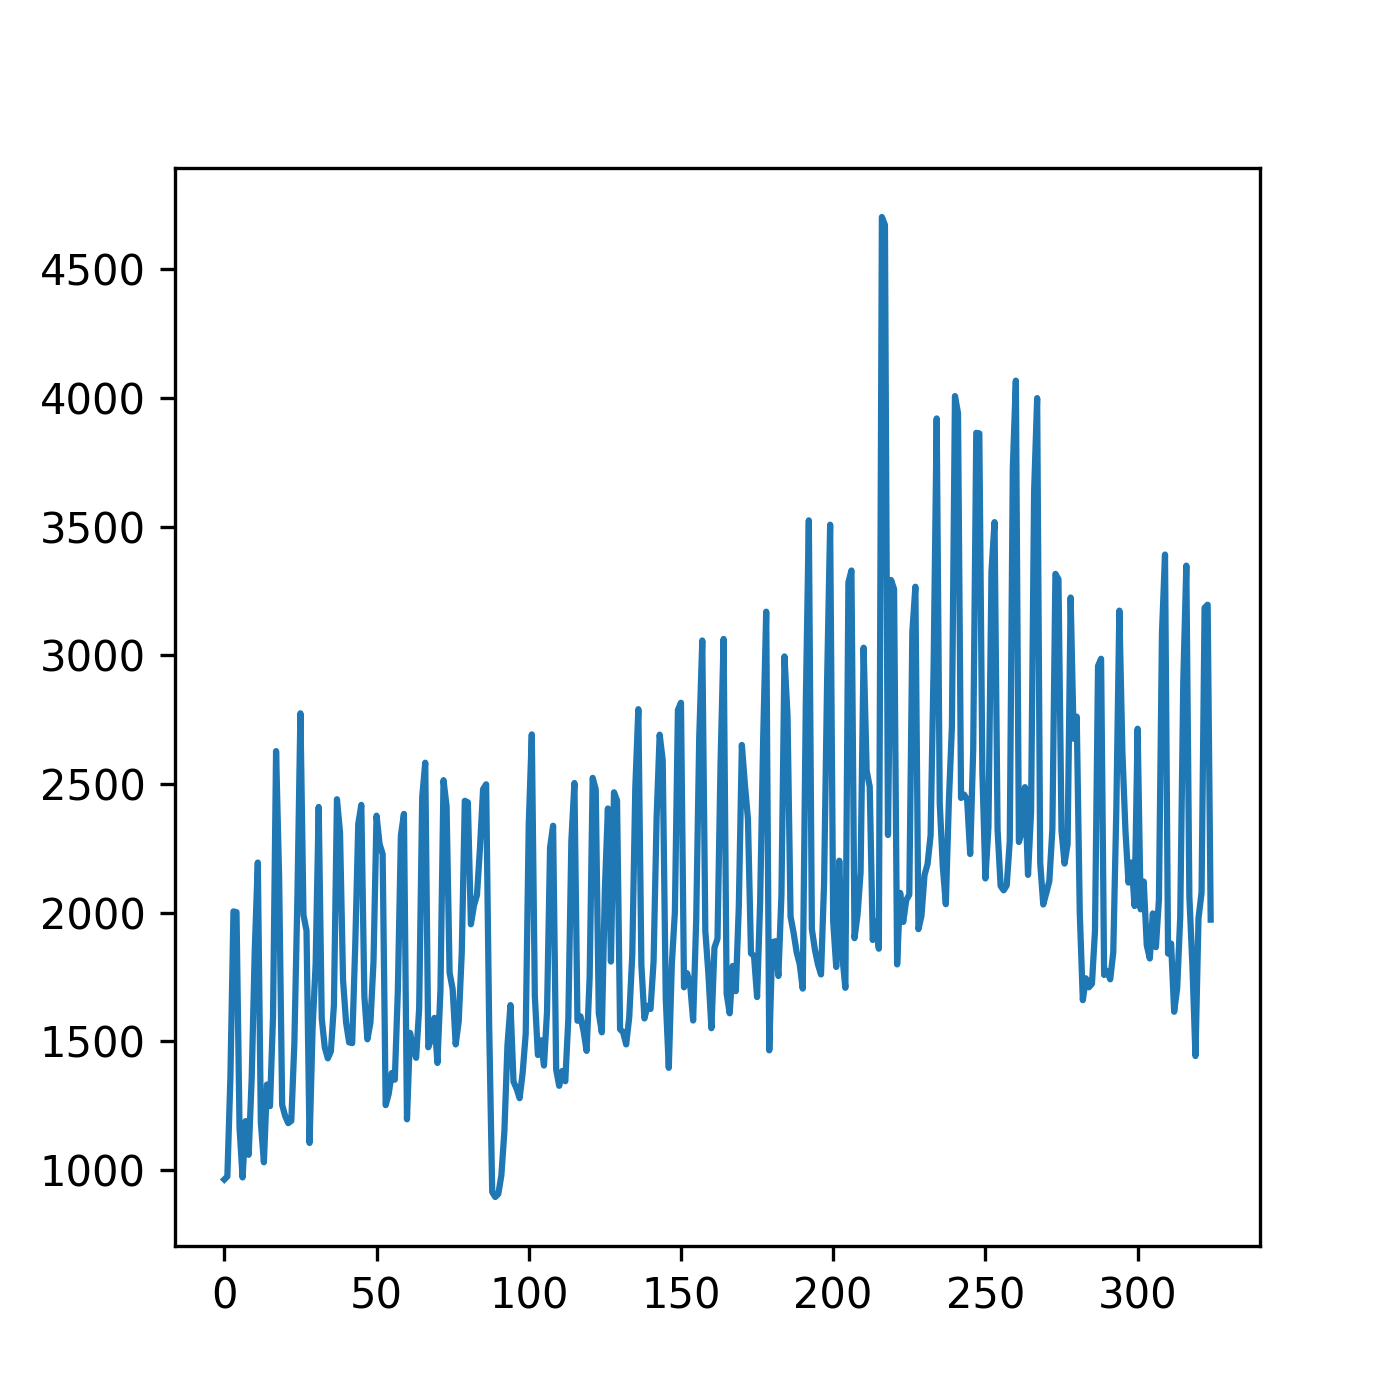
\includegraphics[width=0.75\linewidth]{fig/DailyTransactionVolume.png}
				\caption{Changing of the daily sales volume shows that some features of online sales has been changing all the time. Business transactions shall be checked with the dynamic algorithm.}
				\label{fig:daily-transaction-volume}
			\end{figure}
			
			\begin{figure}[ht]
				\centering
				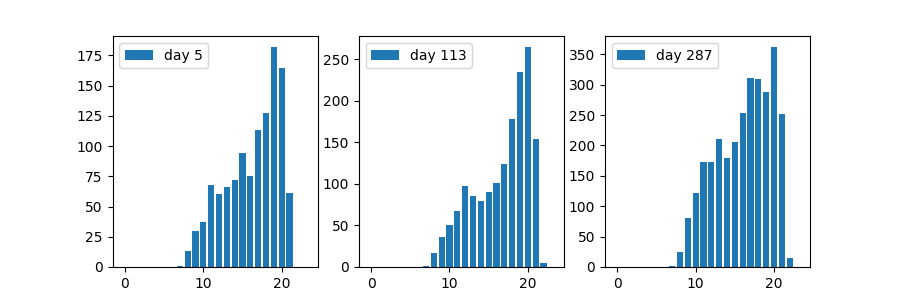
\includegraphics[width=\linewidth]{fig/SaleDistributionSamples.png}
				\caption{We selected 3 days randomly and drew sales distribution by counting hourly volume. Although sales volume has changed from day to day, the shape of the distribution remain almost alike.}
				\label{fig:sale-distribution-sample}
			\end{figure}
			
			Fig.~\ref{fig:daily-transaction-volume} shows the daily transaction volume of the seller. It sees a trend of daily sale which is slightly moving as the time goes. And the daily selling distributions, as is shown in Fig.~\ref{fig:sale-distribution-sample}, display a roughly similar shape.
			
			Click farmed data was generated according to patterns described in section~\ref{sec:related-realworld}. We adopted two prevalent types of click farming: \textit{Centralized Click Farming} and \textit{Equalized Click Farming}. Centralized click farming emulates the scenarios that a group of people are called out and assigned tasks by a casual leader that does not care much about the click farm timing. A significant feature of this approach is that the cheating transactions usually assemble together in a short period of time. Equalized click farming emulates the circumstances that click farms are arranged by some well programmed applications or teams carefully managed and strictly commit transactions according to a timetable. Thus the transaction distribution may not vary too much with and without click farming. According to investigations\textbf{[ref here?]}, the magnitude of click farm varies and depends on the payment the seller can afford. But usually, the click farmed transactions are several times more than the transaction volume it should have. In our experiments, we use $\nu$ to denote the magnitude coefficient of click farm, then $|D_{anomalous}| = (1 + \nu)|D_{normal}|$. In the following experiments without extra illustration, we adopt $\nu = 1$.
			
			To emulate centralized click farming, we randomly inserted some gaussian-distributed transactions in a chosen collection, where the total number of new records is the same of the original volume. As for emulating the equalized click farmers, we simply doubled each record in the chosen collection to make the new distribution exactly the same as the original one, which is harder for the online platform to discover.
			
			To play the role of purchasing platform, we surveillance two levels of transaction distribution. The first level is simply drawing a histogram aligned to time spans. The second level is to draw a histogram on the sub-volumes of each time span. For example, shown in Fig.~\ref{fig:histogram-example}, the first level histogram can be drawn by counting the number of hourly sales. The frequencies of each bucket in 1st level histogram is: $\mathbb{F}=$\{0, 0, 0, 0, 0, 0, 0, 1, 13, 30, 37, 68, 60, 66, 72, 94, 75, 113, 127, 182, 165, 61, 0, 0\}. Then, counting $\mathbb{F}$ with a step size 20 gives the 2nd level histogram.
			
			\begin{figure}[!ht]
				\centering
				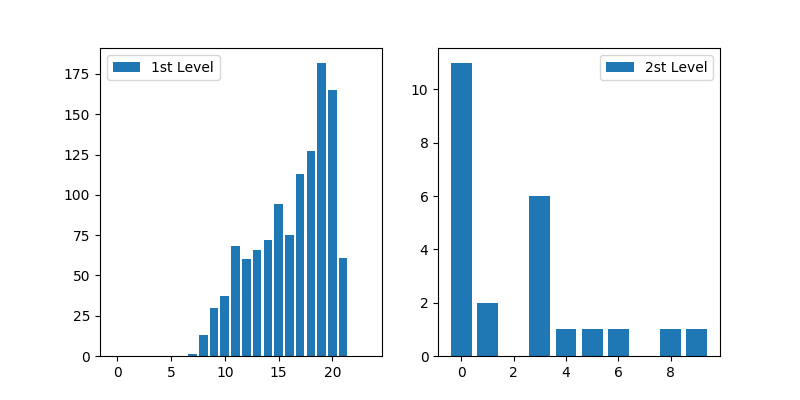
\includegraphics[width=\linewidth]{fig/HistogramExample.png}
				\caption{Example of 1st and 2nd Level Histogram}
				\label{fig:histogram-example}
			\end{figure}
			
			In order to test the performance of Algorithm~\ref{alg:dynamic}, every single collection was fed into the algorithm by the time order. Each collection input has a probability of $\alpha$ to be anomalous, namely, click farmed. The algorithm checks each collection with 1st or 2nd level histogram and give an answer of true or false. Several metrics were explored in the following experiments.
			
		\subsection{Experiment on Raw Data}\label{sec:exp-raw}
			We first tested Algorithm~\ref{alg:dynamic} on raw data set in order to see whether and why the algorithm works. Due to desensitization process, time stamps in raw data set only tell which hour the transaction was committed. Thus, the histogram was drawn by counting hourly volume of each collection. For $\alpha = 0.2$, we select first 30 days as the evidence set of normal collections; day 21st to 30th were also emulated to be click farmed, composing the evidence set of anomalous collections. Equation(9) was employed as the threshold calculator. The results are shown in Table~\ref{tab:result-raw-1st}, where \textit{true positive rate}, \textit{false positive rate} and \textit{accuracy} were recorded.
			
			\begin{table}[!ht]
				\centering
				\caption{Classification Results on Raw Data}
				\label{tab:result-raw-1st}
				\begin{tabular}{|c|c|c|c|c|c|c|}
					\hline
					& \multicolumn{3}{c|}{Centralized} & \multicolumn{3}{c|}{Equalized}\\
					\hline
					& TPR & FAR & ACC & TPR & FAR & ACC\\
					\hline
					1st Level & 100 & 4.05 & 96.72 & 26.64 & 28.03 & 62.49\\
					\hline
					2nd Level & 88.01 & 7.68 & 91.41 & 83.89 & 15.78 & 84.07\\
					\hline
				\end{tabular}
			\end{table}
			
			\begin{figure}[!ht]
				\centering
				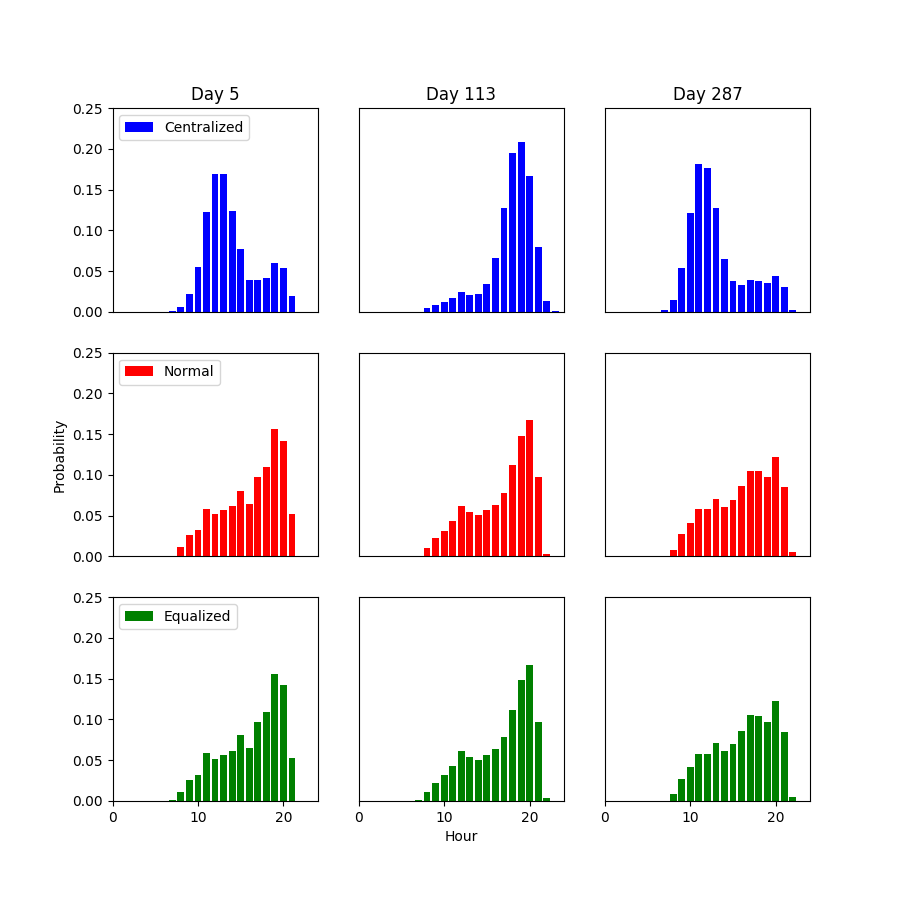
\includegraphics[width=\linewidth]{fig/Raw1stLevelHist.png}
				\caption{1st level histogram of day 5, 113 and 287, each day in a column. Distributions after centralized and equalized click farming are in 1st and 3rd row correspondingly. And the original distributions are shown in 2nd row.}
				\label{fig:raw-hist-1st}
			\end{figure}
			
			\begin{figure}[!ht]
				\centering
				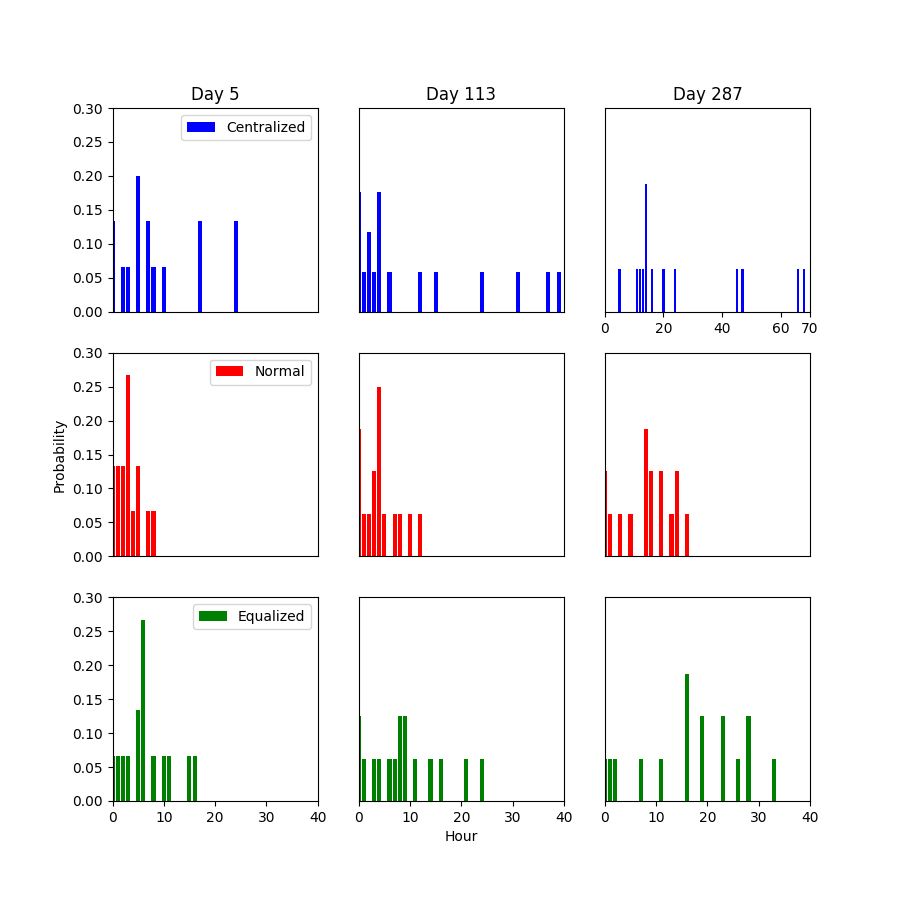
\includegraphics[width=\linewidth]{fig/Raw2ndLevelHist}
				\caption{2nd level histogram of day 5, 113 and 287, each day in a column. Distribution after centralized click farming in day 287 uses another time scale since it deviates a lot from others.}
				\label{fig:raw-hist-2nd}
			\end{figure}
			
			\begin{figure}[!ht]
				\centering
				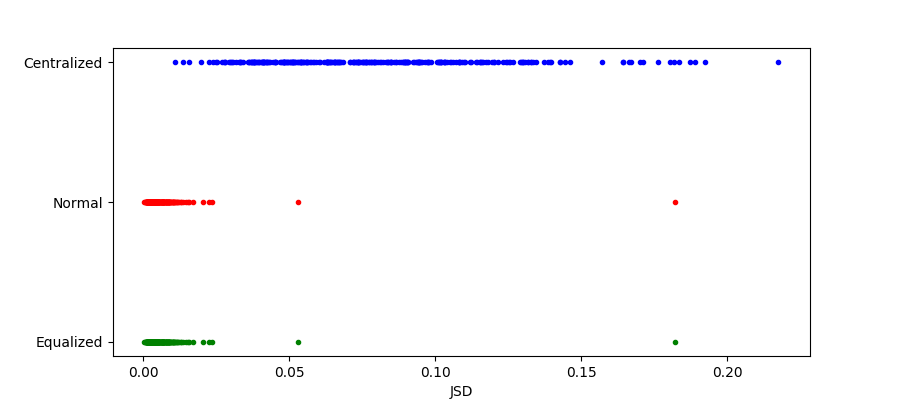
\includegraphics[width=\linewidth]{fig/RawOverview1st.png}
				(a)
				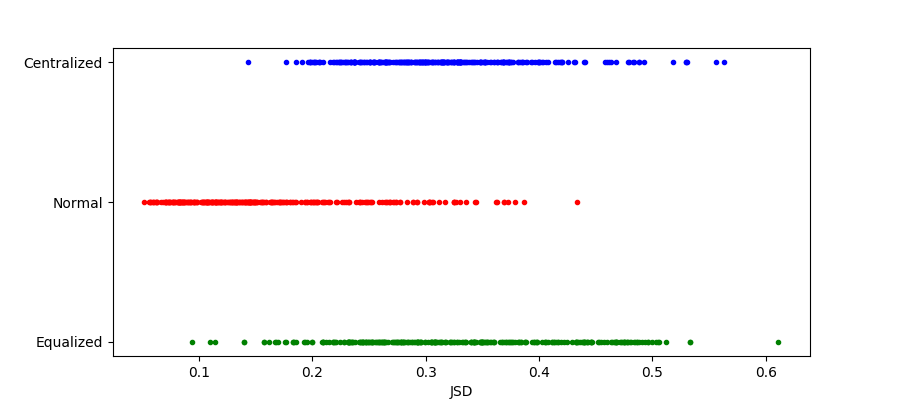
\includegraphics[width=\linewidth]{fig/RawOverview2nd.png}
				(b)
				\caption{This figure shows the JSD values of 1st and 2nd level histogram in each day in three different version: normal, centralized click farmed and equalized click farmed. Both (a) and (b) shows that centralized ones are usually larger than normal ones and most of them clearly distinguishable. In (a), 1st level histogram cannot tell anything different between normal ones and equalized ones. But in (b), 2nd level histograms map the equalized click farmers to the right side of normal ones.}
				\label{fig:raw-overview}
			\end{figure}
			
			When classifying toward 1st level histograms, centralized click farming behaviours can be easily discovered. As displayed in the left two columns in Fig.~\ref{fig:raw-hist-1st}, normal collections share a similar distribution while centralized click farmed ones abruptly violates the original shape. However, as a clever click farmer, equalized click farming did not in the least distorted the distribution. Most of them escaped the security check under the perfect disguise.
			But when it comes to 2nd level histogram, the ``clever disguise'' does not work any longer. It can be clearly seen in Fig.~\ref{fig:raw-hist-2nd} that both types of click farming shows an obvious difference from the normal ones, while the normal ones still share a similar distribution.
			From the overview in Fig.~\ref{fig:raw-overview}, the difference between normal and anomalous collections can be observed more intuitively.
			
		\subsection{Experiment on Synthetic Data}\label{sec:exp-synthetic}
			As is put in the former section, every single record in the transaction set only gives a time stamp aligned at hours. Part of the information was erased with the absence of minutes and seconds. In the following experiments, Every time stamp was assigned a random value for minutes and seconds. Therefore, the synthetic data set should be closer to the real world case. Moreover, the step size in the histograms can now be calculated more precisely. In the 1st level histogram, the constant $c$ in equation(\ref{equ:step-size}) was set to 0.5 since the PDF of daily distribution was approximately a linear function. And in the 2nd level histogram, sub-volumes of every 300 seconds were counted, producing more data points in the 2nd level data collections. Then, constant $c$ in equation(\ref{equ:step-size}) was also set to 0.5 given that the 2nd level histogram was also approximately a linear function.
			We tested algorithm performance for $\alpha \in \{0.1, 0.3, 0.5, 0.7, 0.9\}$, with $E_N$ and $E_A$ the same configuration as before. Results were shown in Table~\ref{tab:syn-result-1st} and~\ref{tab:syn-result-2nd}.
			
			\begin{table}[!ht]
				\centering
				\caption{1st Level}
				\label{tab:syn-result-1st}
				\begin{tabular}{|c|c|c|c|c|c|c|}
					\hline
					& \multicolumn{3}{c|}{Centralized} & \multicolumn{3}{c|}{Equalized}\\
					\hline
					$\alpha$ & TPR(\%) & FPR(\%) & ACC(\%) & TPR(\%) & FPR(\%) & ACC(\%) \\ 
					\hline
					0.1 & 86.10 & 1.14 & 97.40 & 5.75 & 12.28 & 79.66 \\ 
					\hline
					0.2 & 96.43 & 9.83 & 91.30 & 26.97 & 26.47 & 64.29 \\ 
					\hline
					0.3 & 97.95 & 16.49 & 87.68 & 37.46 & 39.46 & 53.67 \\ 
					\hline
					0.4 & 99.18 & 31.94 & 81.30 & 57.23 & 48.32 & 53.79 \\ 
					\hline
					0.5 & 99.33 & 23.40 & 88.25 & 67.67 & 58.23 & 54.46 \\ 
					\hline
					0.6 & 99.62 & 25.70 & 89.83 & 67.03 & 73.78 & 51.64 \\ 
					\hline
					0.7 & 100.00 & 32.51 & 90.51 & 69.69 & 76.28 & 56.16 \\ 
					\hline
					0.8 & 99.72 & 26.97 & 94.35 & 75.56 & 69.44 & 67.00 \\ 
					\hline
					0.9 & 99.63 & 15.73 & 98.19 & 76.59 & 75.18 & 70.73\\
					\hline
				\end{tabular} 
			\end{table}
			
			\begin{table}[!ht]
				\centering
				\caption{2nd Level}
				\label{tab:syn-result-2nd}
				\begin{tabular}{|c|c|c|c|c|c|c|}
					\hline
					& \multicolumn{3}{c|}{Centralized} & \multicolumn{3}{c|}{Equalized}\\
					\hline
					$\alpha$ & TPR(\%) & FPR(\%) & ACC(\%) & TPR(\%) & FPR(\%) & ACC(\%) \\ 
					\hline
					0.1 & 75.60 & 3.90 & 93.74 & 97.84 & 1.64 & 98..31 \\ 
					\hline
					0.2 & 91.93 & 18.43 & 93.73 & 99.42 & 7.39 & 94.01 \\ 
					\hline
					0.3 & 95.01 & 23.70 & 81.69 & 100.00 & 23.93 & 83.05 \\ 
					\hline
					0.4 & 98.09 & 28.66 & 82.49 & 100.00 & 24.59 & 84.75 \\ 
					\hline
					0.5 & 98.33 & 36.54 & 80.00 & 100.00 & 23.76 & 88.36 \\ 
					\hline
					0.6 & 98.35 & 40.69 & 83.41 & 100.00 & 35.94 & 84.63 \\ 
					\hline
					0.7 & 98.54 & 37.97 & 87.80 & 100.00 & 31.27 & 90.84 \\ 
					\hline
					0.8 & 98.47 & 40.38 & 91.19 & 100.00 & 33.04 & 92.66 \\ 
					\hline
					0.9 & 98.51 & 47.56 & 94.58 & 100.00 & 28.44 & 97.40\\
					\hline
				\end{tabular} 
			\end{table}
			
			The result shows that the algorithm can efficiently distinguish the normal and anomalous data collections. No matter how much proportion of data is anomalous, the algorithm always gives a high accuracy. That is because the adaptive threshold was designed to minimize the number of total errors, which was irrelevant to TPR or FPR. When $\alpha$ was increasing, there were less data collections added into $\mathbb{E}_N$. Thus the update of $\mathbb{E}_N$ became slower and FPR went higher. On the contrary, TPR became higher as $\alpha$ increased. Moreover, since $|\mathbb{E}_N| > |\mathbb{E}_A|$, it needs more collection instances for $|\mathbb{E}_N|$ then that for $|\mathbb{E}_A|$ to keep up to the trend. Therefore, it was faster of FPR to increase than TPR to increase. As a result of that, there were more false alarms emerged and ACC went lower, as $\alpha$ increased from 0.1 to 0.5. After that, however, although FPR was still increasing, total number of normal instances decreased dramatically and those false alarms contributed less to total errors. Therefore, ACC rose up again.
			
			\begin{figure}[!ht]
				\centering
				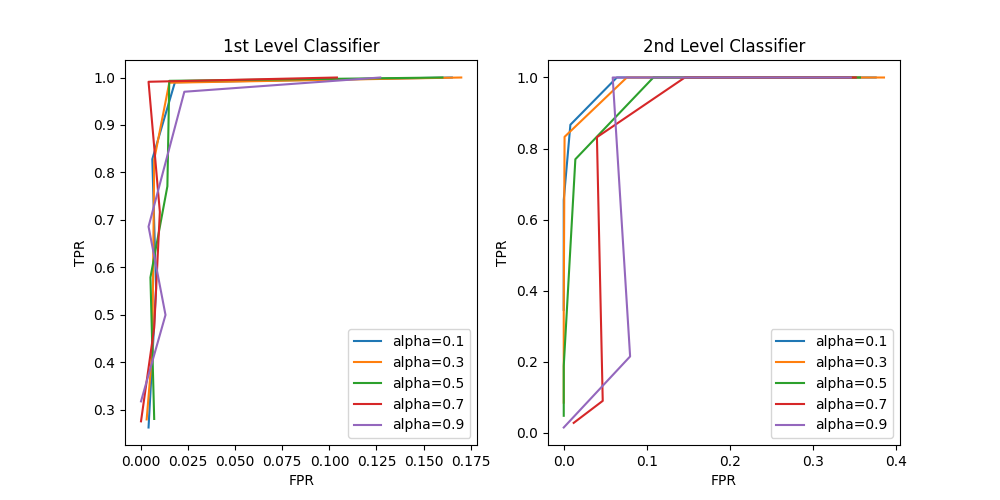
\includegraphics[width=\linewidth]{fig/ROC-Alpha.png}
				\caption{ROC curve of 1st and 2nd level classifier given different values of $\alpha$. The performance of the classifier does not change much for different error rates.}
				\label{fig:roc-alpha}
			\end{figure}
			
			Fig.~\ref{fig:roc-alpha} shows the ROC curve($\nu=1.0$) of the gaussian classifier dealing with centralized click farming with 1st level histograms and equalized manipulation with 2nd level histograms. The curves are pretty close to the upper left corner of the diagram and size under the curves are very large. For different $\alpha$'s, the classifier can efficiently distinguish normal and anomalous data collections.
			
			\begin{figure}[!ht]
				\centering
				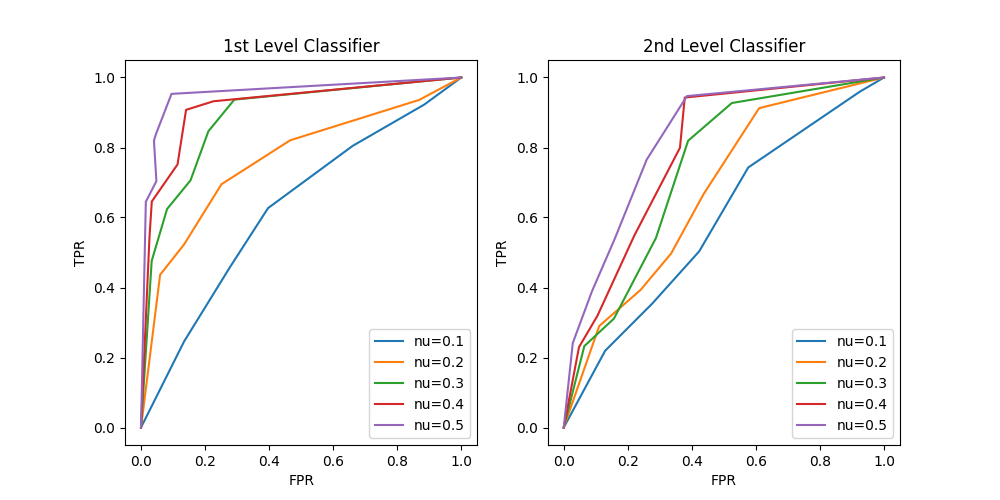
\includegraphics[width=\linewidth]{fig/ROC-Nu.png}
				\caption{ROC curve of different magnitude of click farming. In real world scenarios, $\nu$ is normally larger than 1.}
				\label{fig:roc-magnitude}
			\end{figure}
			
			In Fig.~\ref{fig:roc-magnitude}, we tested the classifier with different magnitude of centralised click farming. In former experiments, the manipulation of centralized click farming always creates as many new transaction records as the original ones. Let $\nu$ denote the magnitude coefficient, then $|D_{anomalous}| = (1 + \nu) |D_{normal}|$. If $\nu $ is smaller, then it will be harder for the classifier to identify anomalous data collections since the anomalous distribution will be closer to normal ones. It can be concluded from the figure that the 1st level classifier can be efficient even when $\nu = 0.3$. However the 2nd level classifier is less sensitive when $\nu = 0.5$. That is because the 1st level histogram provides more probability entries than 2nd level histograms. Data collections are compressed from 1st to 2nd level. But for real world click farming behaviours(usually, $\nu > 1$) both classifiers can be efficient enough.
			
		\subsection{Threshold Optimization}\label{sec:exp-threshold}
			Section~\ref{sec:alg-threshold} mentions only two equations for calculating adaptive thresholds. Table~\ref{tab:threshold-comparison} gives the comparison of more equations out of similar considerations. From the aspect of weighted average(i.e. equation(1)) and taken $\alpha$ into consideration, we composes several other formulas with different operation on $\alpha$ and $\sigma$, yielding other possible balanced points within the interval $[\mu_N, \mu_A]$.
			
			 We tested those calculators on synthetic data set with $\alpha = 0.1, \nu = 1$. Testing each level of classifier and each type of anomalies, we got 4 F1 scores and added them up. Equation 5 gives best performance. Then those equations were tested on large amount of gaussian distributed data instances. 90K and 10K data points were sampled from 500 pairs of random gaussian distributions which represent normal and anomalous distributions respectively, yielding 500 F1 scores for each equation. We compared the average score and discovered that equation 13 gives the best result.
			
			Equation 13 gives best classification result for two gaussian distributions but does not outperform others in real world data. Part of the reasons are mentioned in section~\ref{sec:alg-threshold}. Another reason is that the size of evidence sets are too small, that the gaussian distribution may not be well approximated.
			
			\begin{table*}[!ht]
				\centering
				\caption{F1 Scores of Different Threshold Calculators}
				\label{tab:threshold-comparison}
				\begin{tabular}{|c|c|c|c|}
					\hline
					& Equation & Synthetic & Gaussian \\ 
					\hline
					1 & $\displaystyle T = \frac{\sigma_B \mu_A + \sigma_A \mu_B}{\sigma_B + \sigma_A}$& 1.0588 & 0.5810 \\ 
					\hline
					%2 & $\displaystyle T = \frac{\sqrt{\sigma_B} \mu_A + \sqrt{\sigma_A} \mu_B}{\sqrt{\sigma_B} + \sqrt{\sigma_A}}$& 2.1861 & 0.5718 \\ 
					%\hline
					%3 & $\displaystyle T = \frac{(ln\sigma_B)\mu_A + (ln\sigma_A)\mu_B}{ln\sigma_B + ln\sigma_A}$& 2.2390 & 0.3860 \\ 
					%\hline
					%4 & $\displaystyle T = \frac{(\sqrt{|ln\sigma_B|})\mu_A + (\sqrt{|ln\sigma_A|})\mu_B}{\sqrt{|ln\sigma_B|} + \sqrt{|ln\sigma_A|}}$& 2.2082 & 0.5515 \\ 
					%\hline
					%5 & $\displaystyle T = \frac{(ln\sqrt{\sigma_B})\mu_A + (ln\sqrt{\sigma_A})\mu_B}{ln\sqrt{\sigma_B} + ln\sqrt{\sigma_A}}$& 2.1211 & 0.3811 \\ 
					%\hline
					%\hline
					2 & $\displaystyle T = \frac{\sigma_B (1 - \alpha) \mu_A + \sigma_A \alpha \mu_B}{\sigma_B (1 - \alpha) + \sigma_A \alpha}$& 0.7688 & 0.3515 \\ 
					\hline
					3 & $\displaystyle T = \frac{(\sigma_B \sqrt{1 - \alpha}) \mu_A + (\sigma_A \sqrt{\alpha}) \mu_B}{\sigma_B \sqrt{1 - \alpha} + \sigma_A \sqrt{\alpha}}$& 0.8158 & 0.4510 \\ 
					\hline
					4 & $\displaystyle 
					T = \frac{\big[\sigma_B ln(1 - \alpha)\big] \mu_A
						+ \big[\sigma_A ln\alpha\big] \mu_B}
					{\sigma_B ln(1 - \alpha) + \sigma_A ln\alpha}
					$& 1.5227 & 0.5523 \\ 
					\hline
					5 & $\displaystyle 
					T = \frac{\mu_A \sigma_B \sqrt{-ln(1 - \alpha)}
						+ \mu_B \sigma_A \sqrt{-ln\alpha}}
					{\sigma_B \sqrt{-ln(1 - \alpha)} + \sigma_A \sqrt{-ln\alpha}}
					$& \color{blue}\textbf{2.6013} & 0.5791 \\ 
					\hline
					6 & $\displaystyle 
					T = \frac{\mu_A \sigma_B ln\sqrt{1 - \alpha}
						+ \mu_B \sigma_A ln\sqrt{\alpha}}
					{\sigma_B ln\sqrt{1 - \alpha} + \sigma_A ln\sqrt{\alpha}}
					$& 1.4155 & 0.5578 \\ 
					\hline
					7 & $\displaystyle 
					T = \frac{\mu_A \sqrt{|ln\big[\sigma_B (1 - \alpha)\big]|}
						+ \mu_B \sqrt{|ln(\sigma_A \alpha)|}}
					{\sqrt{|ln\big[\sigma_B (1 - \alpha)\big]|} + \sqrt{|ln(\sigma_A \alpha)|}}
					$& 2.2730 & 0.5600 \\ 
					\hline
					8 & $\displaystyle 
					T = \frac{\mu_A ln\sqrt{\sigma_B (1 - \alpha)}
						+ \mu_B ln\sqrt{\sigma_A \alpha}}
					{ln\sqrt{\sigma_B (1 - \alpha)} + ln\sqrt{\sigma_A \alpha}}
					$& 2.0753 & 0.2808 \\ 
					%\hline
					\hline
					9 & $\displaystyle T = \mathop{\arg\min}_{\mu_A \le T \le \mu_B}\ \alpha \cdot \int_{-\infty}^{T}P_B(x)dx + (1 - \alpha) \cdot \int_{T}^{+\infty}P_A(x)dx$ & 1.9300 & \color{blue}\textbf{0.6072}\\
					\hline
				\end{tabular} 
			\end{table*}
		
		%\subsection{Comparison with other collective classification algorithms}
		%	\textbf{It would be better to have this comparison, but it requires much more experiments and the data set may not be very suitable.}
			
	\section{Conclusion \& Future Work}\label{sec:conclusion}
		This paper proposed an dynamic collective anomaly detection algorithm with adaptive threshold, which helps detect data manipulations in modern data pipelines and data centres. Different from existing algorithms detecting collective anomalies, our approach employs statistical distance as the similarity measurement, mapping data collections to a restricted one dimensional space. We explored several technical points involved in the design of the algorithm and performed a thorough experiment to test its efficiency. It showed that the algorithm can efficiently discover anomalies within the data sequences and the classifier is sensitive enough toward real world data manipulations.
		
		However, the modelling of the JSD distributions is not precise enough. The efficiency of different adaptive thresholds should be tested on different real world circumstances to get a more complete view of their performances. Moreover, a comparison with other collective detection algorithm should be adopted in the future to get an performance overview of similar algorithms. Since the algorithm adapts to the slowly evolving feature, when attacks disguise itself in the long run as if it was one of the changing features, the technique may fail to detect. In this case, other techniques may be applied as assistances.
	
	\section*{Acknowledgement}
		
	\printbibliography
\end{document}




